\chapter{Background}
\label{cha:background}
\section{Constraint Satisfaction Problem}
Constraint Satisfaction Problem(CSP) provides a framework for many various real-life problems in Artificial Intelligence(AI)\cite{r1}\cite{r4}, which is considered as a NP-complete problem. Generally, it consists of 3 parts - Variables (V), Domains (D), and Constraints (C)\cite{r2}\cite{r3}.\\
$\bullet$ V represents a finite set of variables $v_{1}...v_{n}$.\\
$\bullet$ D represents the domains of each variable $D_{v_{1}}.....D_{v_{n}}$.\\
$\bullet$ C is a set of constraints (Here we mainly consider binary constraint:\\ $\{\Constraints{m}{n}\mid v_{m},v_{n}\in v, v_{m}\neq v_{n}\}$ and $\Constraints{m}{n} \in D_{v_{m}} \times D_{v_{n}}$).
\section{Minizinc}
MiniZinc is a constraint modeling language, which is developed by the University of Melbourne, Monash University , and Data61 Decision Sciences\cite{r6}. The minizinc IDE provides a function that transfers the minizinc language to flatzinc language which can be understood by massive solvers\cite{r5}. Meanwhile, it provides some build-in functions as well as optimization methods. In general, the optimizations about minizinc are mainly divided into 2 aspects. One is to optimise the model itself, the other is based on the solvers. For the model itself, the highest level of optimization is arc consistency. Meanwhile, various solvers have different features.
\subsection{Arc Consistency}
According to \cite{r7}, "A variable V is arc consistency with respect to another variable U if and only if for every $d \in D_{v}$ there is at least one $d'\in D_{u}$ such that (d,d') $\in C_{u,v}$". Accordingly, a CSP is arc consistency if and only if all pairs of variables are arc consistency with each other. Based on arc consistency, the values that break arc consistency in the domains will be removed, which significantly decreases the search nodes, at the same time, there is no solution loss. Therefore, it takes up an vital position in CSP.
\subsection{Solver}
As is shown in the figure 1, Flatzinc plays a role of bridge which connects the minizinc with different solvers and correspond interface. A wide range of solvers has supported flatzinc such as Choco, Chuffed, Coin-bc, picatSAT, Gurobi, Jacop, Or-tool, Yuck, Izplus and so on.
\begin{center}
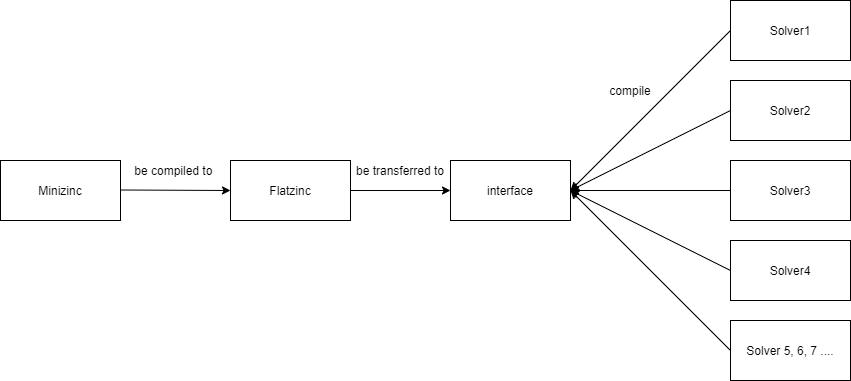
\includegraphics[scale=0.45]{figs/flowofminizinc.png}\\
Fig. 1. The process of solver execute minizinc file
\end{center}
Choco: A JAVA CSP solver, which supports many search strategies( DomWDeg, ABS, IBS, first-fail, etc.) and optimization processes( LNS, fast restart).\\
chuffed: A C++ FD solver using lazy clause generation, which contains a nogood logbook to avoid plenty of duplicate calculation.\\
Coin-bc: A C++ based Mixed Integer Programming (here the MIP model is the same with CSP model) solver, it adopts the branch and cut optimization.\\
picatSAT: A CSP solver based on picat which is a rule-based language. And it adopts log encoding\cite{r8}.\\
Gurobi: A commerical solver support MIP.\\
Jacop: A JAVA CSP solver.\\
Or-tool: An open-source solver developed by google, it combines many optimization methods.\\
Yuck: Based on scala and combines local search with restarting, global constraints, and lexicographic cost functions.\\
Izplus: Based on iZ-C constraint programming that is developed by NTT DATA SEKISUI SYSTEMS CORPORATION. It combines Randomized restarting, Local search, Variable reordering and NG learning.
\section{Rotation Matrix}
Rotation matrix perfectly perform the rotation situations. In this part, we mainly consider the rotations of 90, 180 and 270 degrees for both 2 dimensions and 3 dimensions.
\subsection{2D Rotation Matrix}
The figure 2 shows the 2D rotation matrix, which can imply that $x'=x\cos\theta-y\sin\theta$ and $y'=x\sin\theta+y\cos\theta$. Therefore, if we assign the 90, 180 and 270 degrees to these formulas, we get 3 more situations, 90 degrees (x'=-y,y'=x), 180 degrees (x'=-x, y'=-y) and 270 degrees (x'=y, y'=-x). Usually, in the actual block games, there could appear flip rotations, if flip rotate around x axis, we get  (-x,y) from (x,y), And if flip rotate around y axis, we get(x,-y) from (x,y). If we combine the 2D rotation (90, 180 and 270 degrees) and flip rotation, there are totally 8 situations because (-x,y) rotate 180 degree can get (x,-y), which means there are many duplicates. Therefore, we only need to consider one flip rotate, then it can create 3 more situations based on rotation matrix. 
\begin{center}
$
R(\theta)=\begin{bmatrix}
\cos\theta & -\sin\theta\\
\sin\theta & \cos\theta\\
\end{bmatrix}
$
$\hspace{40pt}$
$
\begin{bmatrix}
x'\\
y'\\
\end{bmatrix}
=\begin{bmatrix}
\cos\theta & -\sin\theta\\
\sin\theta & \cos\theta\\
\end{bmatrix}
\begin{bmatrix}
x\\
y\\
\end{bmatrix}
$
\end{center}
\begin{center}
Fig. 2. 2D rotation matrix
\end{center}
\subsection{3D Rotation Matrix}
Compared to 2D rotation matrix, $R_{z}(\theta)$ (figure 3) is quite similar with 2D rotation matrix. The only difference is that this formula take Z into account. In fact, the general 3D rotation matrix can be decomposed to xy-plane, yz-plane and xz-plane. $R_{z}(\theta)$ is corresponding to xy-plane, that's why it is quite similar with 2D rotation matrix. \\
\begin{center}
$
R_{x}(\theta)=\begin{bmatrix}
1&          0&          0\\
0&\cos\theta & -\sin\theta\\
0&\sin\theta & \cos\theta\\
\end{bmatrix}
$
$\hspace{40pt}$
$
R_{y}(\theta)=\begin{bmatrix}
  \cos\theta&          0&\sin\theta\\
           0&          1& 0\\
-\sin\theta &          0&\cos\theta\\
\end{bmatrix}
$
$
R_{z}(\theta)=\begin{bmatrix}
\cos\theta&-\sin\theta&0\\
\sin\theta& \cos\theta&0\\
         0&          0&1\\
\end{bmatrix}
$\\
\end{center}
\begin{center}
Fig. 3. Basic 3D rotation matrix
\end{center}
Similarly, we only consider 90, 180 and 270 degrees rotation for each plane. Normally, if $R_{x}(\theta)$, $R_{y}(\theta)$ and $R_{z}(\theta)$ are independent, there should be 64 situations because each of them will contains 4 situations. However, according to general rotation matrix (figure 4),
\begin{align*}
&x'=x\cos\alpha\cos\beta+y(\cos\alpha\sin\beta\sin\gamma-\sin\alpha\cos\gamma)+z(\cos\alpha\sin\beta\cos\gamma+\sin\alpha\sin\gamma)\\
&y'=x\sin\alpha\cos\beta+y(\sin\alpha\sin\beta\sin\gamma+\cos\alpha\cos\gamma)+z(\sin\alpha\sin\beta\cos\gamma-\cos\alpha\sin\gamma)\\
&z'=-x\sin\beta+y\cos\beta\sin\gamma+z\cos\beta\cos\gamma
\end{align*}
Obviously, they are not independent. Finally, after eliminate the duplicates, there are total 24 situations.
\begin{center}
$R=R_{x}(\alpha)R_{y}(\beta)R_{z}(\gamma)=
\begin{bmatrix}
\cos\alpha\cos\beta&\cos\alpha\sin\beta\sin\gamma-\sin\alpha\cos\gamma&\cos\alpha\sin\beta\cos\gamma+\sin\alpha\sin\gamma\\
\sin\alpha\cos\beta&\sin\alpha\sin\beta\sin\gamma+\cos\alpha\cos\gamma&\sin\alpha\sin\beta\cos\gamma-\cos\alpha\sin\gamma\\
         -\sin\beta&                               \cos\beta\sin\gamma&\cos\beta\cos\gamma\\
\end{bmatrix}
$
\end{center}
\begin{center}
Fig. 4. General 3D rotation matrix
\end{center}




  


